\documentclass[border=8pt]{standalone}
\usepackage[T1]{fontenc}\usepackage[utf8]{inputenc}\usepackage{lmodern}
\usepackage{tikz}\usetikzlibrary{arrows.meta,positioning}
\begin{document}
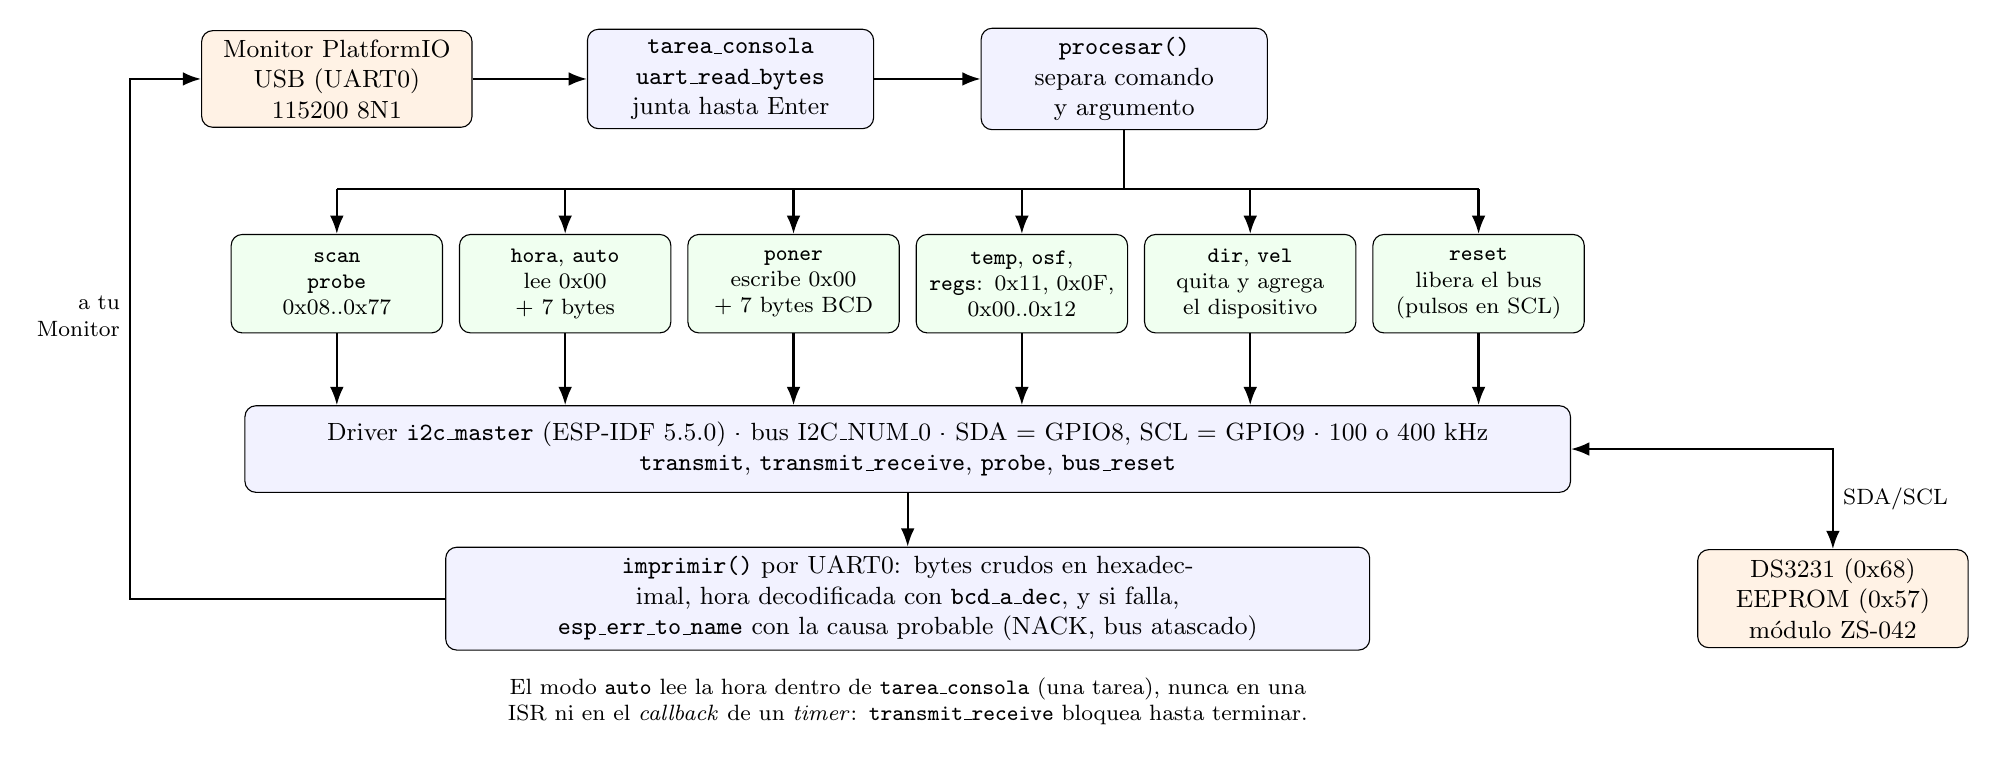
\begin{tikzpicture}[>=Latex,font=\small,
 b/.style={draw,rounded corners,fill=blue!5,align=center,minimum height=1.1cm},
 h/.style={draw,rounded corners,fill=orange!10,align=center,minimum height=1.1cm,text width=3.2cm},
 c/.style={draw,rounded corners,fill=green!6,text width=2.45cm,align=center,minimum height=1.25cm,font=\footnotesize}]
% fila 1: entrada de comandos
\node[h] (mon) at (0,0) {Monitor PlatformIO\\USB (UART0)\\115200 8N1};
\node[b,text width=3.4cm] (rx) at (5.0,0) {\texttt{tarea\_consola}\\\texttt{uart\_read\_bytes}\\junta hasta Enter};
\node[b,text width=3.4cm] (pr) at (10.0,0) {\texttt{procesar()}\\separa comando\\y argumento};
\draw[->,thick] (mon)--(rx); \draw[->,thick] (rx)--(pr);
% fila 2: comandos
\foreach \x/\n/\t in {0/c1/{\texttt{scan}\\\texttt{probe}\\0x08..0x77},
                      2.9/c2/{\texttt{hora}, \texttt{auto}\\lee 0x00\\+ 7 bytes},
                      5.8/c3/{\texttt{poner}\\escribe 0x00\\+ 7 bytes BCD},
                      8.7/c4/{\texttt{temp}, \texttt{osf},\\\texttt{regs}: 0x11, 0x0F,\\0x00..0x12},
                      11.6/c5/{\texttt{dir}, \texttt{vel}\\quita y agrega\\el dispositivo},
                      14.5/c6/{\texttt{reset}\\libera el bus\\(pulsos en SCL)}}
  \node[c] (\n) at (\x,-2.6) {\t};
\draw[thick] (pr.south) -- (10.0,-1.4);
\draw[thick] (0,-1.4) -- (14.5,-1.4);
\foreach \n in {c1,c2,c3,c4,c5,c6} \draw[->,thick] (\n |- 0,-1.4) -- (\n.north);
% fila 3: driver y chip
\node[b,text width=16.6cm] (drv) at (7.25,-4.7) {Driver \texttt{i2c\_master} (ESP-IDF 5.5.0) · bus I2C\_NUM\_0 · SDA = GPIO8, SCL = GPIO9 · 100 o 400 kHz\\\texttt{transmit}, \texttt{transmit\_receive}, \texttt{probe}, \texttt{bus\_reset}};
\foreach \n in {c1,c2,c3,c4,c5,c6} \draw[->,thick] (\n.south) -- (\n |- drv.north);
\node[h] (rtc) at (19.0,-6.6) {DS3231 (0x68)\\EEPROM (0x57)\\módulo ZS-042};
\draw[<->,thick] (drv.east) -| node[pos=0.75,right,font=\footnotesize]{SDA/SCL} (rtc.north);
% fila 4: salida
\node[b,text width=11.5cm] (out) at (7.25,-6.6) {\texttt{imprimir()} por UART0: bytes crudos en hexadecimal, hora decodificada con \texttt{bcd\_a\_dec}, y si falla, \texttt{esp\_err\_to\_name} con la causa probable (NACK, bus atascado)};
\draw[->,thick] (drv.south) -- (out.north);
\draw[->,thick] (out.west) -| node[pos=0.8,left,font=\footnotesize,align=right]{a tu\\Monitor} ([xshift=-0.9cm]mon.south west) -- ([xshift=-0.9cm]mon.south west |- mon.west) -- (mon.west);
\node[font=\footnotesize,text width=17cm,align=center] at (7.25,-7.9) {El modo \texttt{auto} lee la hora dentro de \texttt{tarea\_consola} (una tarea), nunca en una ISR ni en el \emph{callback} de un \emph{timer}: \texttt{transmit\_receive} bloquea hasta terminar.};
\end{tikzpicture}
\end{document}
